% Created by tikzDevice version 0.7.0 on 2014-11-06 12:23:31
% !TEX encoding = UTF-8 Unicode
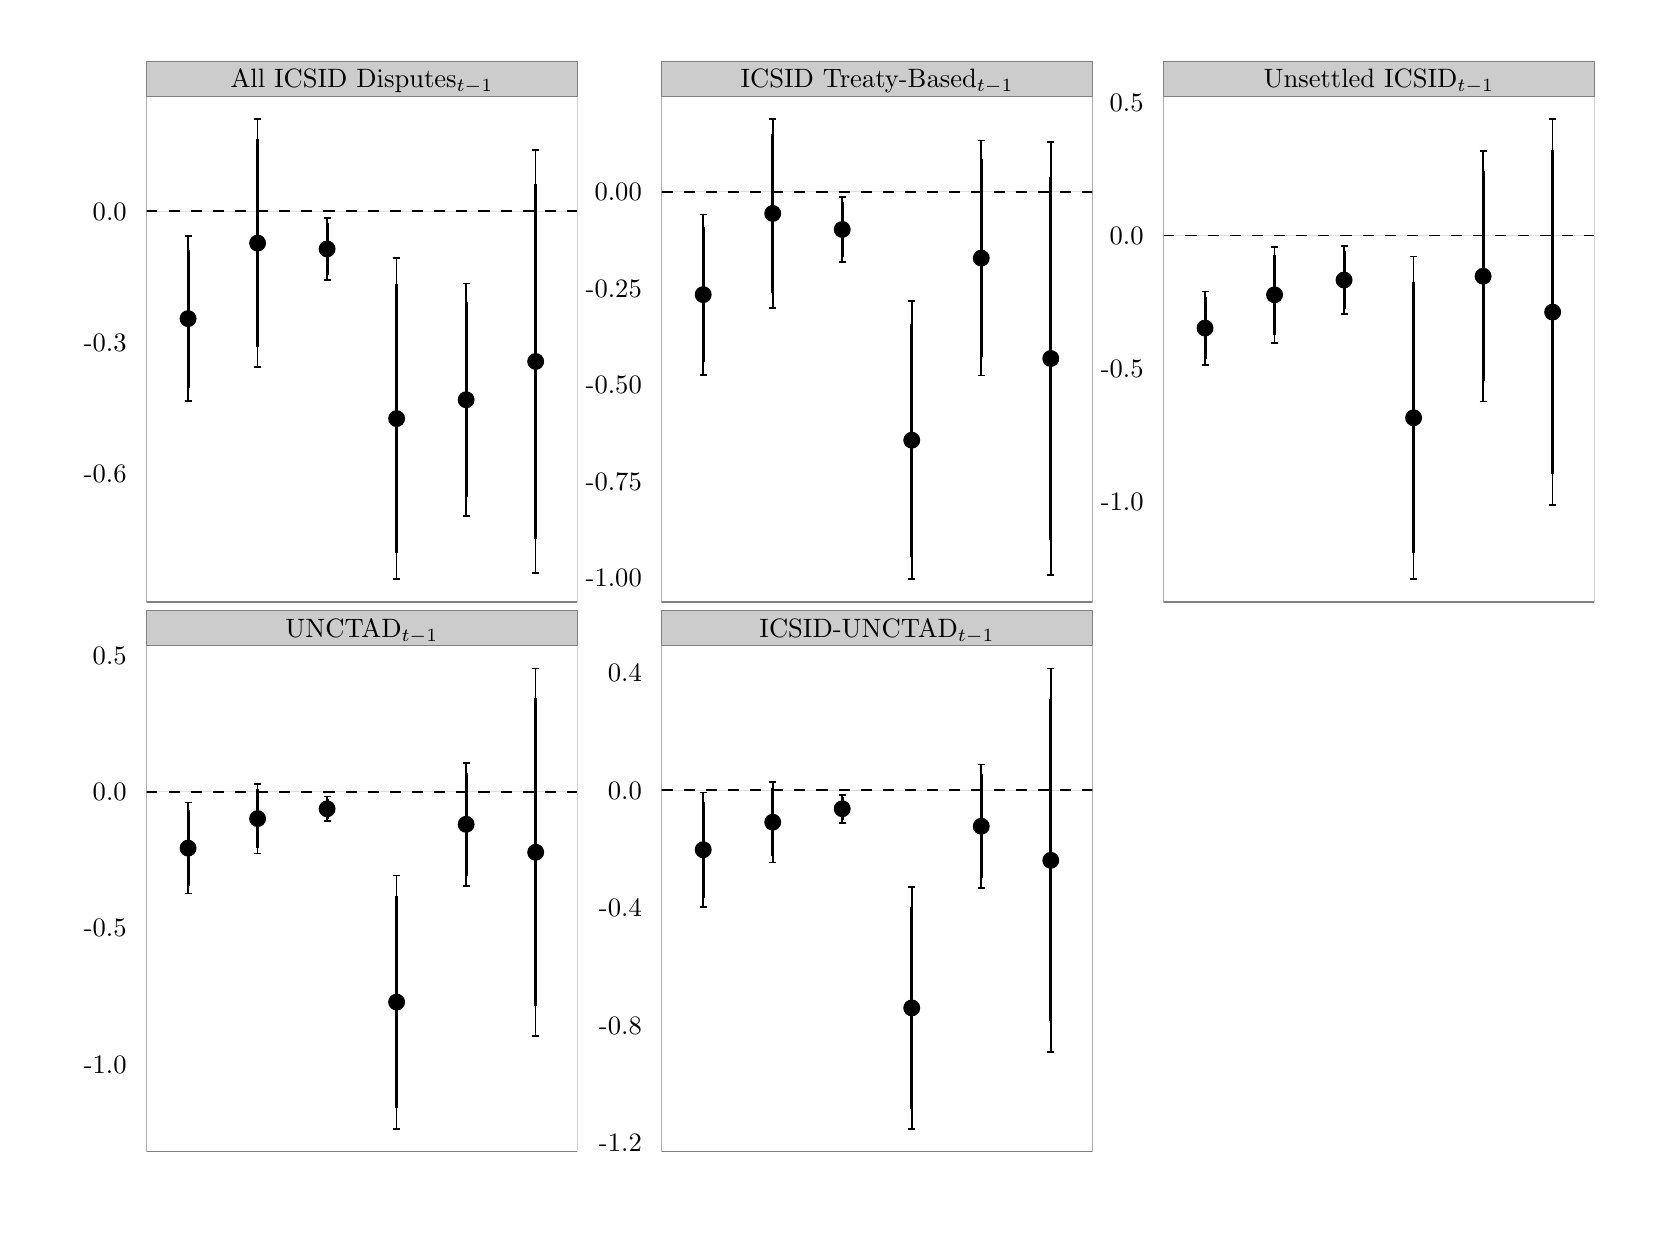
\begin{tikzpicture}[x=1pt,y=1pt]
\definecolor[named]{fillColor}{rgb}{1.00,1.00,1.00}
\path[use as bounding box,fill=fillColor,fill opacity=0.00] (0,0) rectangle (578.16,433.62);
\begin{scope}
\path[clip] (  0.00,  0.00) rectangle (578.16,433.62);
\definecolor[named]{drawColor}{rgb}{1.00,1.00,1.00}
\definecolor[named]{fillColor}{rgb}{1.00,1.00,1.00}

\path[draw=drawColor,line width= 0.6pt,line join=round,line cap=round,fill=fillColor] (  0.00,  0.00) rectangle (578.16,433.62);
\end{scope}
\begin{scope}
\path[clip] ( 42.89,226.00) rectangle (198.64,408.94);
\definecolor[named]{fillColor}{rgb}{1.00,1.00,1.00}

\path[fill=fillColor] ( 42.89,226.00) rectangle (198.64,408.94);
\definecolor[named]{drawColor}{rgb}{0.00,0.00,0.00}
\definecolor[named]{fillColor}{rgb}{0.00,0.00,0.00}

\path[draw=drawColor,draw opacity=0.30,line width= 0.3pt,line join=round,fill=fillColor,fill opacity=0.30] ( 57.96,298.73) -- ( 57.96,358.23);

\path[draw=drawColor,draw opacity=0.30,line width= 0.3pt,line join=round,fill=fillColor,fill opacity=0.30] ( 83.08,310.91) -- ( 83.08,400.63);

\path[draw=drawColor,draw opacity=0.30,line width= 0.3pt,line join=round,fill=fillColor,fill opacity=0.30] (108.20,342.51) -- (108.20,364.81);

\path[draw=drawColor,draw opacity=0.30,line width= 0.3pt,line join=round,fill=fillColor,fill opacity=0.30] (133.32,234.32) -- (133.32,350.41);

\path[draw=drawColor,draw opacity=0.30,line width= 0.3pt,line join=round,fill=fillColor,fill opacity=0.30] (158.44,257.14) -- (158.44,341.19);

\path[draw=drawColor,draw opacity=0.30,line width= 0.3pt,line join=round,fill=fillColor,fill opacity=0.30] (183.56,236.47) -- (183.56,389.53);
\definecolor[named]{drawColor}{rgb}{0.00,0.00,0.00}
\definecolor[named]{fillColor}{rgb}{0.00,0.00,0.00}

\path[draw=drawColor,line width= 1.1pt,line join=round,fill=fillColor] ( 57.96,303.51) -- ( 57.96,353.45);

\path[draw=drawColor,line width= 1.1pt,line join=round,fill=fillColor] ( 83.08,318.12) -- ( 83.08,393.41);

\path[draw=drawColor,line width= 1.1pt,line join=round,fill=fillColor] (108.20,344.30) -- (108.20,363.02);

\path[draw=drawColor,line width= 1.1pt,line join=round,fill=fillColor] (133.32,243.65) -- (133.32,341.08);

\path[draw=drawColor,line width= 1.1pt,line join=round,fill=fillColor] (158.44,263.90) -- (158.44,334.43);

\path[draw=drawColor,line width= 1.1pt,line join=round,fill=fillColor] (183.56,248.77) -- (183.56,377.22);

\path[draw=drawColor,line width= 0.6pt,dash pattern=on 4pt off 4pt ,line join=round,fill=fillColor] ( 42.89,367.26) -- (198.64,367.26);

\path[draw=drawColor,line width= 0.4pt,line join=round,line cap=round,fill=fillColor] ( 57.96,328.48) circle (  2.85);

\path[draw=drawColor,line width= 0.4pt,line join=round,line cap=round,fill=fillColor] ( 83.08,355.77) circle (  2.85);

\path[draw=drawColor,line width= 0.4pt,line join=round,line cap=round,fill=fillColor] (108.20,353.66) circle (  2.85);

\path[draw=drawColor,line width= 0.4pt,line join=round,line cap=round,fill=fillColor] (133.32,292.36) circle (  2.85);

\path[draw=drawColor,line width= 0.4pt,line join=round,line cap=round,fill=fillColor] (158.44,299.16) circle (  2.85);

\path[draw=drawColor,line width= 0.4pt,line join=round,line cap=round,fill=fillColor] (183.56,313.00) circle (  2.85);

\path[draw=drawColor,line width= 0.6pt,line join=round] ( 56.70,358.23) --
	( 59.21,358.23);

\path[draw=drawColor,line width= 0.6pt,line join=round] ( 57.96,358.23) --
	( 57.96,298.73);

\path[draw=drawColor,line width= 0.6pt,line join=round] ( 56.70,298.73) --
	( 59.21,298.73);

\path[draw=drawColor,line width= 0.6pt,line join=round] ( 81.82,400.63) --
	( 84.34,400.63);

\path[draw=drawColor,line width= 0.6pt,line join=round] ( 83.08,400.63) --
	( 83.08,310.91);

\path[draw=drawColor,line width= 0.6pt,line join=round] ( 81.82,310.91) --
	( 84.34,310.91);

\path[draw=drawColor,line width= 0.6pt,line join=round] (106.95,364.81) --
	(109.46,364.81);

\path[draw=drawColor,line width= 0.6pt,line join=round] (108.20,364.81) --
	(108.20,342.51);

\path[draw=drawColor,line width= 0.6pt,line join=round] (106.95,342.51) --
	(109.46,342.51);

\path[draw=drawColor,line width= 0.6pt,line join=round] (132.07,350.41) --
	(134.58,350.41);

\path[draw=drawColor,line width= 0.6pt,line join=round] (133.32,350.41) --
	(133.32,234.32);

\path[draw=drawColor,line width= 0.6pt,line join=round] (132.07,234.32) --
	(134.58,234.32);

\path[draw=drawColor,line width= 0.6pt,line join=round] (157.19,341.19) --
	(159.70,341.19);

\path[draw=drawColor,line width= 0.6pt,line join=round] (158.44,341.19) --
	(158.44,257.14);

\path[draw=drawColor,line width= 0.6pt,line join=round] (157.19,257.14) --
	(159.70,257.14);

\path[draw=drawColor,line width= 0.6pt,line join=round] (182.31,389.53) --
	(184.82,389.53);

\path[draw=drawColor,line width= 0.6pt,line join=round] (183.56,389.53) --
	(183.56,236.47);

\path[draw=drawColor,line width= 0.6pt,line join=round] (182.31,236.47) --
	(184.82,236.47);
\definecolor[named]{drawColor}{rgb}{0.50,0.50,0.50}

\path[draw=drawColor,line width= 0.6pt,line join=round,line cap=round] ( 42.89,226.00) rectangle (198.64,408.94);
\end{scope}
\begin{scope}
\path[clip] (229.02,226.00) rectangle (384.78,408.94);
\definecolor[named]{fillColor}{rgb}{1.00,1.00,1.00}

\path[fill=fillColor] (229.02,226.00) rectangle (384.78,408.94);
\definecolor[named]{drawColor}{rgb}{0.00,0.00,0.00}
\definecolor[named]{fillColor}{rgb}{0.00,0.00,0.00}

\path[draw=drawColor,draw opacity=0.30,line width= 0.3pt,line join=round,fill=fillColor,fill opacity=0.30] (244.10,308.17) -- (244.10,366.14);

\path[draw=drawColor,draw opacity=0.30,line width= 0.3pt,line join=round,fill=fillColor,fill opacity=0.30] (269.22,332.36) -- (269.22,400.63);

\path[draw=drawColor,draw opacity=0.30,line width= 0.3pt,line join=round,fill=fillColor,fill opacity=0.30] (294.34,348.89) -- (294.34,372.51);

\path[draw=drawColor,draw opacity=0.30,line width= 0.3pt,line join=round,fill=fillColor,fill opacity=0.30] (319.46,234.32) -- (319.46,334.78);

\path[draw=drawColor,draw opacity=0.30,line width= 0.3pt,line join=round,fill=fillColor,fill opacity=0.30] (344.58,307.87) -- (344.58,392.83);

\path[draw=drawColor,draw opacity=0.30,line width= 0.3pt,line join=round,fill=fillColor,fill opacity=0.30] (369.70,235.73) -- (369.70,392.42);
\definecolor[named]{drawColor}{rgb}{0.00,0.00,0.00}
\definecolor[named]{fillColor}{rgb}{0.00,0.00,0.00}

\path[draw=drawColor,line width= 1.1pt,line join=round,fill=fillColor] (244.10,312.83) -- (244.10,361.48);

\path[draw=drawColor,line width= 1.1pt,line join=round,fill=fillColor] (269.22,337.85) -- (269.22,395.14);

\path[draw=drawColor,line width= 1.1pt,line join=round,fill=fillColor] (294.34,350.79) -- (294.34,370.61);

\path[draw=drawColor,line width= 1.1pt,line join=round,fill=fillColor] (319.46,242.40) -- (319.46,326.71);

\path[draw=drawColor,line width= 1.1pt,line join=round,fill=fillColor] (344.58,314.70) -- (344.58,386.00);

\path[draw=drawColor,line width= 1.1pt,line join=round,fill=fillColor] (369.70,248.32) -- (369.70,379.82);

\path[draw=drawColor,line width= 0.6pt,dash pattern=on 4pt off 4pt ,line join=round,fill=fillColor] (229.02,374.30) -- (384.78,374.30);

\path[draw=drawColor,line width= 0.4pt,line join=round,line cap=round,fill=fillColor] (244.10,337.15) circle (  2.85);

\path[draw=drawColor,line width= 0.4pt,line join=round,line cap=round,fill=fillColor] (269.22,366.49) circle (  2.85);

\path[draw=drawColor,line width= 0.4pt,line join=round,line cap=round,fill=fillColor] (294.34,360.70) circle (  2.85);

\path[draw=drawColor,line width= 0.4pt,line join=round,line cap=round,fill=fillColor] (319.46,284.55) circle (  2.85);

\path[draw=drawColor,line width= 0.4pt,line join=round,line cap=round,fill=fillColor] (344.58,350.35) circle (  2.85);

\path[draw=drawColor,line width= 0.4pt,line join=round,line cap=round,fill=fillColor] (369.70,314.07) circle (  2.85);

\path[draw=drawColor,line width= 0.6pt,line join=round] (242.84,366.14) --
	(245.35,366.14);

\path[draw=drawColor,line width= 0.6pt,line join=round] (244.10,366.14) --
	(244.10,308.17);

\path[draw=drawColor,line width= 0.6pt,line join=round] (242.84,308.17) --
	(245.35,308.17);

\path[draw=drawColor,line width= 0.6pt,line join=round] (267.96,400.63) --
	(270.47,400.63);

\path[draw=drawColor,line width= 0.6pt,line join=round] (269.22,400.63) --
	(269.22,332.36);

\path[draw=drawColor,line width= 0.6pt,line join=round] (267.96,332.36) --
	(270.47,332.36);

\path[draw=drawColor,line width= 0.6pt,line join=round] (293.08,372.51) --
	(295.60,372.51);

\path[draw=drawColor,line width= 0.6pt,line join=round] (294.34,372.51) --
	(294.34,348.89);

\path[draw=drawColor,line width= 0.6pt,line join=round] (293.08,348.89) --
	(295.60,348.89);

\path[draw=drawColor,line width= 0.6pt,line join=round] (318.20,334.78) --
	(320.72,334.78);

\path[draw=drawColor,line width= 0.6pt,line join=round] (319.46,334.78) --
	(319.46,234.32);

\path[draw=drawColor,line width= 0.6pt,line join=round] (318.20,234.32) --
	(320.72,234.32);

\path[draw=drawColor,line width= 0.6pt,line join=round] (343.33,392.83) --
	(345.84,392.83);

\path[draw=drawColor,line width= 0.6pt,line join=round] (344.58,392.83) --
	(344.58,307.87);

\path[draw=drawColor,line width= 0.6pt,line join=round] (343.33,307.87) --
	(345.84,307.87);

\path[draw=drawColor,line width= 0.6pt,line join=round] (368.45,392.42) --
	(370.96,392.42);

\path[draw=drawColor,line width= 0.6pt,line join=round] (369.70,392.42) --
	(369.70,235.73);

\path[draw=drawColor,line width= 0.6pt,line join=round] (368.45,235.73) --
	(370.96,235.73);
\definecolor[named]{drawColor}{rgb}{0.50,0.50,0.50}

\path[draw=drawColor,line width= 0.6pt,line join=round,line cap=round] (229.02,226.00) rectangle (384.78,408.94);
\end{scope}
\begin{scope}
\path[clip] (410.36,226.00) rectangle (566.12,408.94);
\definecolor[named]{fillColor}{rgb}{1.00,1.00,1.00}

\path[fill=fillColor] (410.36,226.00) rectangle (566.12,408.94);
\definecolor[named]{drawColor}{rgb}{0.00,0.00,0.00}
\definecolor[named]{fillColor}{rgb}{0.00,0.00,0.00}

\path[draw=drawColor,draw opacity=0.30,line width= 0.3pt,line join=round,fill=fillColor,fill opacity=0.30] (425.44,311.84) -- (425.44,338.31);

\path[draw=drawColor,draw opacity=0.30,line width= 0.3pt,line join=round,fill=fillColor,fill opacity=0.30] (450.56,319.74) -- (450.56,354.44);

\path[draw=drawColor,draw opacity=0.30,line width= 0.3pt,line join=round,fill=fillColor,fill opacity=0.30] (475.68,330.07) -- (475.68,354.79);

\path[draw=drawColor,draw opacity=0.30,line width= 0.3pt,line join=round,fill=fillColor,fill opacity=0.30] (500.80,234.32) -- (500.80,350.97);

\path[draw=drawColor,draw opacity=0.30,line width= 0.3pt,line join=round,fill=fillColor,fill opacity=0.30] (525.92,298.53) -- (525.92,389.06);

\path[draw=drawColor,draw opacity=0.30,line width= 0.3pt,line join=round,fill=fillColor,fill opacity=0.30] (551.04,261.03) -- (551.04,400.63);
\definecolor[named]{drawColor}{rgb}{0.00,0.00,0.00}
\definecolor[named]{fillColor}{rgb}{0.00,0.00,0.00}

\path[draw=drawColor,line width= 1.1pt,line join=round,fill=fillColor] (425.44,313.97) -- (425.44,336.18);

\path[draw=drawColor,line width= 1.1pt,line join=round,fill=fillColor] (450.56,322.53) -- (450.56,351.65);

\path[draw=drawColor,line width= 1.1pt,line join=round,fill=fillColor] (475.68,332.06) -- (475.68,352.81);

\path[draw=drawColor,line width= 1.1pt,line join=round,fill=fillColor] (500.80,243.70) -- (500.80,341.59);

\path[draw=drawColor,line width= 1.1pt,line join=round,fill=fillColor] (525.92,305.81) -- (525.92,381.78);

\path[draw=drawColor,line width= 1.1pt,line join=round,fill=fillColor] (551.04,272.25) -- (551.04,389.40);

\path[draw=drawColor,line width= 0.6pt,dash pattern=on 4pt off 4pt ,line join=round,fill=fillColor] (410.36,358.47) -- (566.12,358.47);

\path[draw=drawColor,line width= 0.4pt,line join=round,line cap=round,fill=fillColor] (425.44,325.07) circle (  2.85);

\path[draw=drawColor,line width= 0.4pt,line join=round,line cap=round,fill=fillColor] (450.56,337.09) circle (  2.85);

\path[draw=drawColor,line width= 0.4pt,line join=round,line cap=round,fill=fillColor] (475.68,342.43) circle (  2.85);

\path[draw=drawColor,line width= 0.4pt,line join=round,line cap=round,fill=fillColor] (500.80,292.65) circle (  2.85);

\path[draw=drawColor,line width= 0.4pt,line join=round,line cap=round,fill=fillColor] (525.92,343.80) circle (  2.85);

\path[draw=drawColor,line width= 0.4pt,line join=round,line cap=round,fill=fillColor] (551.04,330.83) circle (  2.85);

\path[draw=drawColor,line width= 0.6pt,line join=round] (424.18,338.31) --
	(426.69,338.31);

\path[draw=drawColor,line width= 0.6pt,line join=round] (425.44,338.31) --
	(425.44,311.84);

\path[draw=drawColor,line width= 0.6pt,line join=round] (424.18,311.84) --
	(426.69,311.84);

\path[draw=drawColor,line width= 0.6pt,line join=round] (449.30,354.44) --
	(451.81,354.44);

\path[draw=drawColor,line width= 0.6pt,line join=round] (450.56,354.44) --
	(450.56,319.74);

\path[draw=drawColor,line width= 0.6pt,line join=round] (449.30,319.74) --
	(451.81,319.74);

\path[draw=drawColor,line width= 0.6pt,line join=round] (474.42,354.79) --
	(476.93,354.79);

\path[draw=drawColor,line width= 0.6pt,line join=round] (475.68,354.79) --
	(475.68,330.07);

\path[draw=drawColor,line width= 0.6pt,line join=round] (474.42,330.07) --
	(476.93,330.07);

\path[draw=drawColor,line width= 0.6pt,line join=round] (499.54,350.97) --
	(502.06,350.97);

\path[draw=drawColor,line width= 0.6pt,line join=round] (500.80,350.97) --
	(500.80,234.32);

\path[draw=drawColor,line width= 0.6pt,line join=round] (499.54,234.32) --
	(502.06,234.32);

\path[draw=drawColor,line width= 0.6pt,line join=round] (524.66,389.06) --
	(527.18,389.06);

\path[draw=drawColor,line width= 0.6pt,line join=round] (525.92,389.06) --
	(525.92,298.53);

\path[draw=drawColor,line width= 0.6pt,line join=round] (524.66,298.53) --
	(527.18,298.53);

\path[draw=drawColor,line width= 0.6pt,line join=round] (549.79,400.63) --
	(552.30,400.63);

\path[draw=drawColor,line width= 0.6pt,line join=round] (551.04,400.63) --
	(551.04,261.03);

\path[draw=drawColor,line width= 0.6pt,line join=round] (549.79,261.03) --
	(552.30,261.03);
\definecolor[named]{drawColor}{rgb}{0.50,0.50,0.50}

\path[draw=drawColor,line width= 0.6pt,line join=round,line cap=round] (410.36,226.00) rectangle (566.12,408.94);
\end{scope}
\begin{scope}
\path[clip] ( 42.89, 27.42) rectangle (198.64,210.36);
\definecolor[named]{fillColor}{rgb}{1.00,1.00,1.00}

\path[fill=fillColor] ( 42.89, 27.42) rectangle (198.64,210.36);
\definecolor[named]{drawColor}{rgb}{0.00,0.00,0.00}
\definecolor[named]{fillColor}{rgb}{0.00,0.00,0.00}

\path[draw=drawColor,draw opacity=0.30,line width= 0.3pt,line join=round,fill=fillColor,fill opacity=0.30] ( 57.96,120.70) -- ( 57.96,153.59);

\path[draw=drawColor,draw opacity=0.30,line width= 0.3pt,line join=round,fill=fillColor,fill opacity=0.30] ( 83.08,135.25) -- ( 83.08,160.39);

\path[draw=drawColor,draw opacity=0.30,line width= 0.3pt,line join=round,fill=fillColor,fill opacity=0.30] (108.20,146.92) -- (108.20,155.77);

\path[draw=drawColor,draw opacity=0.30,line width= 0.3pt,line join=round,fill=fillColor,fill opacity=0.30] (133.32, 35.74) -- (133.32,127.30);

\path[draw=drawColor,draw opacity=0.30,line width= 0.3pt,line join=round,fill=fillColor,fill opacity=0.30] (158.44,123.52) -- (158.44,167.98);

\path[draw=drawColor,draw opacity=0.30,line width= 0.3pt,line join=round,fill=fillColor,fill opacity=0.30] (183.56, 69.24) -- (183.56,202.04);
\definecolor[named]{drawColor}{rgb}{0.00,0.00,0.00}
\definecolor[named]{fillColor}{rgb}{0.00,0.00,0.00}

\path[draw=drawColor,line width= 1.1pt,line join=round,fill=fillColor] ( 57.96,123.35) -- ( 57.96,150.95);

\path[draw=drawColor,line width= 1.1pt,line join=round,fill=fillColor] ( 83.08,137.27) -- ( 83.08,158.37);

\path[draw=drawColor,line width= 1.1pt,line join=round,fill=fillColor] (108.20,147.63) -- (108.20,155.06);

\path[draw=drawColor,line width= 1.1pt,line join=round,fill=fillColor] (133.32, 43.10) -- (133.32,119.94);

\path[draw=drawColor,line width= 1.1pt,line join=round,fill=fillColor] (158.44,127.09) -- (158.44,164.40);

\path[draw=drawColor,line width= 1.1pt,line join=round,fill=fillColor] (183.56, 79.92) -- (183.56,191.37);

\path[draw=drawColor,line width= 0.6pt,dash pattern=on 4pt off 4pt ,line join=round,fill=fillColor] ( 42.89,157.52) -- (198.64,157.52);

\path[draw=drawColor,line width= 0.4pt,line join=round,line cap=round,fill=fillColor] ( 57.96,137.15) circle (  2.85);

\path[draw=drawColor,line width= 0.4pt,line join=round,line cap=round,fill=fillColor] ( 83.08,147.82) circle (  2.85);

\path[draw=drawColor,line width= 0.4pt,line join=round,line cap=round,fill=fillColor] (108.20,151.35) circle (  2.85);

\path[draw=drawColor,line width= 0.4pt,line join=round,line cap=round,fill=fillColor] (133.32, 81.52) circle (  2.85);

\path[draw=drawColor,line width= 0.4pt,line join=round,line cap=round,fill=fillColor] (158.44,145.75) circle (  2.85);

\path[draw=drawColor,line width= 0.4pt,line join=round,line cap=round,fill=fillColor] (183.56,135.64) circle (  2.85);

\path[draw=drawColor,line width= 0.6pt,line join=round] ( 56.70,153.59) --
	( 59.21,153.59);

\path[draw=drawColor,line width= 0.6pt,line join=round] ( 57.96,153.59) --
	( 57.96,120.70);

\path[draw=drawColor,line width= 0.6pt,line join=round] ( 56.70,120.70) --
	( 59.21,120.70);

\path[draw=drawColor,line width= 0.6pt,line join=round] ( 81.82,160.39) --
	( 84.34,160.39);

\path[draw=drawColor,line width= 0.6pt,line join=round] ( 83.08,160.39) --
	( 83.08,135.25);

\path[draw=drawColor,line width= 0.6pt,line join=round] ( 81.82,135.25) --
	( 84.34,135.25);

\path[draw=drawColor,line width= 0.6pt,line join=round] (106.95,155.77) --
	(109.46,155.77);

\path[draw=drawColor,line width= 0.6pt,line join=round] (108.20,155.77) --
	(108.20,146.92);

\path[draw=drawColor,line width= 0.6pt,line join=round] (106.95,146.92) --
	(109.46,146.92);

\path[draw=drawColor,line width= 0.6pt,line join=round] (132.07,127.30) --
	(134.58,127.30);

\path[draw=drawColor,line width= 0.6pt,line join=round] (133.32,127.30) --
	(133.32, 35.74);

\path[draw=drawColor,line width= 0.6pt,line join=round] (132.07, 35.74) --
	(134.58, 35.74);

\path[draw=drawColor,line width= 0.6pt,line join=round] (157.19,167.98) --
	(159.70,167.98);

\path[draw=drawColor,line width= 0.6pt,line join=round] (158.44,167.98) --
	(158.44,123.52);

\path[draw=drawColor,line width= 0.6pt,line join=round] (157.19,123.52) --
	(159.70,123.52);

\path[draw=drawColor,line width= 0.6pt,line join=round] (182.31,202.04) --
	(184.82,202.04);

\path[draw=drawColor,line width= 0.6pt,line join=round] (183.56,202.04) --
	(183.56, 69.24);

\path[draw=drawColor,line width= 0.6pt,line join=round] (182.31, 69.24) --
	(184.82, 69.24);
\definecolor[named]{drawColor}{rgb}{0.50,0.50,0.50}

\path[draw=drawColor,line width= 0.6pt,line join=round,line cap=round] ( 42.89, 27.42) rectangle (198.64,210.36);
\end{scope}
\begin{scope}
\path[clip] (229.02, 27.42) rectangle (384.78,210.36);
\definecolor[named]{fillColor}{rgb}{1.00,1.00,1.00}

\path[fill=fillColor] (229.02, 27.42) rectangle (384.78,210.36);
\definecolor[named]{drawColor}{rgb}{0.00,0.00,0.00}
\definecolor[named]{fillColor}{rgb}{0.00,0.00,0.00}

\path[draw=drawColor,draw opacity=0.30,line width= 0.3pt,line join=round,fill=fillColor,fill opacity=0.30] (244.10,115.89) -- (244.10,157.25);

\path[draw=drawColor,draw opacity=0.30,line width= 0.3pt,line join=round,fill=fillColor,fill opacity=0.30] (269.22,131.98) -- (269.22,161.06);

\path[draw=drawColor,draw opacity=0.30,line width= 0.3pt,line join=round,fill=fillColor,fill opacity=0.30] (294.34,146.33) -- (294.34,156.42);

\path[draw=drawColor,draw opacity=0.30,line width= 0.3pt,line join=round,fill=fillColor,fill opacity=0.30] (319.46, 35.74) -- (319.46,123.07);

\path[draw=drawColor,draw opacity=0.30,line width= 0.3pt,line join=round,fill=fillColor,fill opacity=0.30] (344.58,122.70) -- (344.58,167.41);

\path[draw=drawColor,draw opacity=0.30,line width= 0.3pt,line join=round,fill=fillColor,fill opacity=0.30] (369.70, 63.44) -- (369.70,202.04);
\definecolor[named]{drawColor}{rgb}{0.00,0.00,0.00}
\definecolor[named]{fillColor}{rgb}{0.00,0.00,0.00}

\path[draw=drawColor,line width= 1.1pt,line join=round,fill=fillColor] (244.10,119.22) -- (244.10,153.93);

\path[draw=drawColor,line width= 1.1pt,line join=round,fill=fillColor] (269.22,134.32) -- (269.22,158.72);

\path[draw=drawColor,line width= 1.1pt,line join=round,fill=fillColor] (294.34,147.14) -- (294.34,155.61);

\path[draw=drawColor,line width= 1.1pt,line join=round,fill=fillColor] (319.46, 42.76) -- (319.46,116.05);

\path[draw=drawColor,line width= 1.1pt,line join=round,fill=fillColor] (344.58,126.29) -- (344.58,163.82);

\path[draw=drawColor,line width= 1.1pt,line join=round,fill=fillColor] (369.70, 74.58) -- (369.70,190.90);

\path[draw=drawColor,line width= 0.6pt,dash pattern=on 4pt off 4pt ,line join=round,fill=fillColor] (229.02,158.05) -- (384.78,158.05);

\path[draw=drawColor,line width= 0.4pt,line join=round,line cap=round,fill=fillColor] (244.10,136.57) circle (  2.85);

\path[draw=drawColor,line width= 0.4pt,line join=round,line cap=round,fill=fillColor] (269.22,146.52) circle (  2.85);

\path[draw=drawColor,line width= 0.4pt,line join=round,line cap=round,fill=fillColor] (294.34,151.38) circle (  2.85);

\path[draw=drawColor,line width= 0.4pt,line join=round,line cap=round,fill=fillColor] (319.46, 79.41) circle (  2.85);

\path[draw=drawColor,line width= 0.4pt,line join=round,line cap=round,fill=fillColor] (344.58,145.05) circle (  2.85);

\path[draw=drawColor,line width= 0.4pt,line join=round,line cap=round,fill=fillColor] (369.70,132.74) circle (  2.85);

\path[draw=drawColor,line width= 0.6pt,line join=round] (242.84,157.25) --
	(245.35,157.25);

\path[draw=drawColor,line width= 0.6pt,line join=round] (244.10,157.25) --
	(244.10,115.89);

\path[draw=drawColor,line width= 0.6pt,line join=round] (242.84,115.89) --
	(245.35,115.89);

\path[draw=drawColor,line width= 0.6pt,line join=round] (267.96,161.06) --
	(270.47,161.06);

\path[draw=drawColor,line width= 0.6pt,line join=round] (269.22,161.06) --
	(269.22,131.98);

\path[draw=drawColor,line width= 0.6pt,line join=round] (267.96,131.98) --
	(270.47,131.98);

\path[draw=drawColor,line width= 0.6pt,line join=round] (293.08,156.42) --
	(295.60,156.42);

\path[draw=drawColor,line width= 0.6pt,line join=round] (294.34,156.42) --
	(294.34,146.33);

\path[draw=drawColor,line width= 0.6pt,line join=round] (293.08,146.33) --
	(295.60,146.33);

\path[draw=drawColor,line width= 0.6pt,line join=round] (318.20,123.07) --
	(320.72,123.07);

\path[draw=drawColor,line width= 0.6pt,line join=round] (319.46,123.07) --
	(319.46, 35.74);

\path[draw=drawColor,line width= 0.6pt,line join=round] (318.20, 35.74) --
	(320.72, 35.74);

\path[draw=drawColor,line width= 0.6pt,line join=round] (343.33,167.41) --
	(345.84,167.41);

\path[draw=drawColor,line width= 0.6pt,line join=round] (344.58,167.41) --
	(344.58,122.70);

\path[draw=drawColor,line width= 0.6pt,line join=round] (343.33,122.70) --
	(345.84,122.70);

\path[draw=drawColor,line width= 0.6pt,line join=round] (368.45,202.04) --
	(370.96,202.04);

\path[draw=drawColor,line width= 0.6pt,line join=round] (369.70,202.04) --
	(369.70, 63.44);

\path[draw=drawColor,line width= 0.6pt,line join=round] (368.45, 63.44) --
	(370.96, 63.44);
\definecolor[named]{drawColor}{rgb}{0.50,0.50,0.50}

\path[draw=drawColor,line width= 0.6pt,line join=round,line cap=round] (229.02, 27.42) rectangle (384.78,210.36);
\end{scope}
\begin{scope}
\path[clip] (  0.00,  0.00) rectangle (578.16,433.62);
\definecolor[named]{drawColor}{rgb}{0.50,0.50,0.50}
\definecolor[named]{fillColor}{rgb}{0.80,0.80,0.80}

\path[draw=drawColor,line width= 0.2pt,line join=round,line cap=round,fill=fillColor] ( 42.89,408.94) rectangle (198.64,421.57);
\definecolor[named]{drawColor}{rgb}{0.00,0.00,0.00}

\node[text=drawColor,anchor=base,inner sep=0pt, outer sep=0pt, scale=  0.96] at (120.76,411.95) {All ICSID Disputes$_{t-1}$};
\end{scope}
\begin{scope}
\path[clip] (  0.00,  0.00) rectangle (578.16,433.62);
\definecolor[named]{drawColor}{rgb}{0.50,0.50,0.50}
\definecolor[named]{fillColor}{rgb}{0.80,0.80,0.80}

\path[draw=drawColor,line width= 0.2pt,line join=round,line cap=round,fill=fillColor] (229.02,408.94) rectangle (384.78,421.57);
\definecolor[named]{drawColor}{rgb}{0.00,0.00,0.00}

\node[text=drawColor,anchor=base,inner sep=0pt, outer sep=0pt, scale=  0.96] at (306.90,411.95) {ICSID Treaty-Based$_{t-1}$};
\end{scope}
\begin{scope}
\path[clip] (  0.00,  0.00) rectangle (578.16,433.62);
\definecolor[named]{drawColor}{rgb}{0.50,0.50,0.50}
\definecolor[named]{fillColor}{rgb}{0.80,0.80,0.80}

\path[draw=drawColor,line width= 0.2pt,line join=round,line cap=round,fill=fillColor] (410.36,408.94) rectangle (566.12,421.57);
\definecolor[named]{drawColor}{rgb}{0.00,0.00,0.00}

\node[text=drawColor,anchor=base,inner sep=0pt, outer sep=0pt, scale=  0.96] at (488.24,411.95) {Unsettled ICSID$_{t-1}$};
\end{scope}
\begin{scope}
\path[clip] (  0.00,  0.00) rectangle (578.16,433.62);
\definecolor[named]{drawColor}{rgb}{0.50,0.50,0.50}
\definecolor[named]{fillColor}{rgb}{0.80,0.80,0.80}

\path[draw=drawColor,line width= 0.2pt,line join=round,line cap=round,fill=fillColor] ( 42.89,210.36) rectangle (198.64,222.99);
\definecolor[named]{drawColor}{rgb}{0.00,0.00,0.00}

\node[text=drawColor,anchor=base,inner sep=0pt, outer sep=0pt, scale=  0.96] at (120.76,213.37) {UNCTAD$_{t-1}$};
\end{scope}
\begin{scope}
\path[clip] (  0.00,  0.00) rectangle (578.16,433.62);
\definecolor[named]{drawColor}{rgb}{0.50,0.50,0.50}
\definecolor[named]{fillColor}{rgb}{0.80,0.80,0.80}

\path[draw=drawColor,line width= 0.2pt,line join=round,line cap=round,fill=fillColor] (229.02,210.36) rectangle (384.78,222.99);
\definecolor[named]{drawColor}{rgb}{0.00,0.00,0.00}

\node[text=drawColor,anchor=base,inner sep=0pt, outer sep=0pt, scale=  0.96] at (306.90,213.37) {ICSID-UNCTAD$_{t-1}$};
\end{scope}
\begin{scope}
\path[clip] (  0.00,  0.00) rectangle (578.16,433.62);
\definecolor[named]{drawColor}{rgb}{0.00,0.00,0.00}

\node[text=drawColor,anchor=base east,inner sep=0pt, outer sep=0pt, scale=  0.96] at ( 35.77,269.17) {-0.6};

\node[text=drawColor,anchor=base east,inner sep=0pt, outer sep=0pt, scale=  0.96] at ( 35.77,316.56) {-0.3};

\node[text=drawColor,anchor=base east,inner sep=0pt, outer sep=0pt, scale=  0.96] at ( 35.77,363.96) {0.0};
\end{scope}
\begin{scope}
\path[clip] (  0.00,  0.00) rectangle (578.16,433.62);
\definecolor[named]{drawColor}{rgb}{0.00,0.00,0.00}

\node[text=drawColor,anchor=base east,inner sep=0pt, outer sep=0pt, scale=  0.96] at (221.91,231.52) {-1.00};

\node[text=drawColor,anchor=base east,inner sep=0pt, outer sep=0pt, scale=  0.96] at (221.91,266.38) {-0.75};

\node[text=drawColor,anchor=base east,inner sep=0pt, outer sep=0pt, scale=  0.96] at (221.91,301.25) {-0.50};

\node[text=drawColor,anchor=base east,inner sep=0pt, outer sep=0pt, scale=  0.96] at (221.91,336.12) {-0.25};

\node[text=drawColor,anchor=base east,inner sep=0pt, outer sep=0pt, scale=  0.96] at (221.91,370.99) {0.00};
\end{scope}
\begin{scope}
\path[clip] (  0.00,  0.00) rectangle (578.16,433.62);
\definecolor[named]{drawColor}{rgb}{0.00,0.00,0.00}

\node[text=drawColor,anchor=base east,inner sep=0pt, outer sep=0pt, scale=  0.96] at (403.25,258.97) {-1.0};

\node[text=drawColor,anchor=base east,inner sep=0pt, outer sep=0pt, scale=  0.96] at (403.25,307.07) {-0.5};

\node[text=drawColor,anchor=base east,inner sep=0pt, outer sep=0pt, scale=  0.96] at (403.25,355.17) {0.0};

\node[text=drawColor,anchor=base east,inner sep=0pt, outer sep=0pt, scale=  0.96] at (403.25,403.27) {0.5};
\end{scope}
\begin{scope}
\path[clip] (  0.00,  0.00) rectangle (578.16,433.62);
\definecolor[named]{drawColor}{rgb}{0.00,0.00,0.00}

\node[text=drawColor,anchor=base east,inner sep=0pt, outer sep=0pt, scale=  0.96] at ( 35.77, 55.86) {-1.0};

\node[text=drawColor,anchor=base east,inner sep=0pt, outer sep=0pt, scale=  0.96] at ( 35.77,105.04) {-0.5};

\node[text=drawColor,anchor=base east,inner sep=0pt, outer sep=0pt, scale=  0.96] at ( 35.77,154.22) {0.0};

\node[text=drawColor,anchor=base east,inner sep=0pt, outer sep=0pt, scale=  0.96] at ( 35.77,203.40) {0.5};
\end{scope}
\begin{scope}
\path[clip] (  0.00,  0.00) rectangle (578.16,433.62);
\definecolor[named]{drawColor}{rgb}{0.00,0.00,0.00}

\node[text=drawColor,anchor=base east,inner sep=0pt, outer sep=0pt, scale=  0.96] at (221.91, 27.39) {-1.2};

\node[text=drawColor,anchor=base east,inner sep=0pt, outer sep=0pt, scale=  0.96] at (221.91, 69.84) {-0.8};

\node[text=drawColor,anchor=base east,inner sep=0pt, outer sep=0pt, scale=  0.96] at (221.91,112.29) {-0.4};

\node[text=drawColor,anchor=base east,inner sep=0pt, outer sep=0pt, scale=  0.96] at (221.91,154.75) {0.0};

\node[text=drawColor,anchor=base east,inner sep=0pt, outer sep=0pt, scale=  0.96] at (221.91,197.20) {0.4};
\end{scope}
\end{tikzpicture}
